\documentclass[11pt,a4paper]{report}

% ---------- Encoding & fonts ----------
\usepackage[utf8]{inputenc}
\usepackage[T1]{fontenc}
\usepackage{lmodern}

% ---------- Math & symbols ----------
\usepackage{amsmath,amssymb,amsthm}

% ---------- Page layout ----------
\usepackage{geometry}
\geometry{
  margin=1in
}

% ---------- Spacing ----------
\usepackage{setspace}
\onehalfspacing

% ---------- Graphics & figures ----------
\usepackage{graphicx}
\usepackage{xcolor}
\usepackage{tikz}
\usetikzlibrary{arrows.meta, positioning, shapes.geometric}

% ---------- Hyperlinks ----------
\usepackage[hidelinks]{hyperref}

% ---------- Better lists ----------
\usepackage{enumitem}

% ---------- For code / pseudo-code (optional) ----------
\usepackage{listings}
\lstset{
  basicstyle=\ttfamily\small,
  breaklines=true,
  frame=single
}

% ---------- Theorem environments ----------
\newtheorem{theorem}{Theorem}[section]
\newtheorem{lemma}[theorem]{Lemma}
\newtheorem{proposition}[theorem]{Proposition}
\newtheorem{corollary}[theorem]{Corollary}
\theoremstyle{definition}
\newtheorem{definition}[theorem]{Definition}
\newtheorem{example}[theorem]{Example}
\theoremstyle{remark}
\newtheorem{remark}[theorem]{Remark}

% ---------- Document metadata ----------
\title{HUM{\Large$\Lambda$}N-Ø Protocol Whitepaper\\[4pt]
       \large Proof of Sustainable Humanity (PoSH)}
\author{Edward Calderón et al.}
\date{\today}

\begin{document}

\maketitle

\begin{center}
  Contact: \texttt{contact@human0.me}
\end{center}

\tableofcontents
\clearpage

% =====================================================
% Manifesto (1-page, more technical / crypto-oriented)
% =====================================================

\chapter*{Manifesto}
\addcontentsline{toc}{chapter}{Manifesto}

Humanity is simultaneously running two non-linear processes: an accelerating
planetary crisis and an expanding digital infrastructure largely indifferent to
physical limits. The systems that secure our digital assets today---hashpower,
stake, and centralized identity---do not secure our future on this planet.

HUM{\Large$\Lambda$}N-Ø begins from a simple assertion: sustainability must
become a \emph{first-class cryptographic primitive}. Our digital identities
should not only prove ownership or solvency, but also attest to our contribution
to planetary stability. We call this primitive \textbf{Proof of Sustainable
Humanity (PoSH)}.

Traditional consensus:

\begin{itemize}[leftmargin=*]
  \item \emph{Proof of Work} consumes energy as a Sybil-resistance mechanism;
        its security budget is paid in thermodynamic cost.
  \item \emph{Proof of Stake} concentrates control in capital and remains
        structurally agnostic to real-world emissions or ecological impact.
\end{itemize}

Neither model encodes a notion of \emph{human-scale, positive environmental
action}. They secure ledgers; they do not secure the biosphere.

HUM{\Large$\Lambda$}N-Ø proposes a complementary axis of trust: a ledger in
which each entry corresponds to a verifiable sustainability event attributed to
a unique human. Measurement, reporting, and verification (MRV) pipelines
generate signed records of renewable energy use, low-carbon mobility, or
regenerative actions. Oracle networks transform these records into
cryptographically committed claims. Zero-knowledge proofs \cite{GMR85} allow individuals to
demonstrate that they have performed valid actions according to public
methodologies, without exposing their raw behavioral data.

At the core of PoSH is a simple mapping:
\[
  \text{Human} \;\rightarrow\; \mathsf{humanId} \;\rightarrow\;
  \{\text{impact commitments on-chain}\}.
\]
Each commitment is an immutable binding between a pseudonymous human identifier
and an attested sustainability event, derived as a hash of MRV data, methodology
references, and oracle attestations. Together, these commitments form a
sustainability ledger keyed by human beings, not by accounts or corporations.

The protocol is non-extractive by design. Minting a PoSH proof must cost no more
than the underlying network fee. No central party is entitled to rent-seek on
the right of a human to demonstrate positive impact. The economic incentives are
shifted: it is rational to invest in better MRV, in higher-quality oracles, and
in more transparent methodologies, but not to charge individuals for access to
their own sustainability record.

We affirm the following:

\begin{itemize}[leftmargin=*]
  \item Every human should be able to hold a cryptographic proof of their
        positive environmental actions.
  \item These proofs must be verifiable without requiring the disclosure of
        private life details.
  \item The infrastructure to mint and verify such proofs must be open,
        composable, and globally accessible.
  \item No governance, market, or institution should be able to monopolize or
        censor the representation of sustainable humanity.
\end{itemize}

HUM{\Large$\Lambda$}N-Ø does not claim to solve climate change. It aims to
provide the minimal cryptographic substrate on which more honest, transparent,
and human-scale climate coordination can be built. By embedding sustainability
directly into identity and state, we align digital verification with ecological
reality.

Zero is not an absence; it is a boundary condition. Net zero is not a slogan,
but a statement that can---and must---be proven. HUM{\Large$\Lambda$}N-Ø is an
invitation to treat that proof as a public good.

\clearpage

% =====================================================
% PoSH Chapter (technical architecture)
% =====================================================

\chapter{Proof of Sustainable Humanity (PoSH)}
\label{chap:posh}

\section{Introduction}

The accelerating climate crisis reveals a structural gap in how digital systems
recognize, value, and verify human contributions to environmental sustainability.
Existing blockchain consensus mechanisms---such as Proof of Work (PoW) and Proof
of Stake (PoS)---are fundamentally unsuitable for representing or incentivizing
human-scale sustainable action. PoW externalizes environmental cost through
computational waste \cite{goodell2020greenBlockchain}, while PoS concentrates power among capital-rich actors and
remains detached from real-world impact \cite{saleh2021pos}.

\textbf{Proof of Sustainable Humanity (PoSH)} is introduced as a new primitive:
a cryptographically verifiable, privacy-preserving mechanism that represents the
positive, measurable environmental actions performed by unique human individuals.
PoSH is designed as the foundational trust layer of the HUM{\Large$\Lambda$}N-Ø
protocol, enabling transparent, decentralized verification of sustainability
actions without requiring invasive identification or resource-intensive
computation.

Prior initiatives in proof-of-personhood and decentralized identity highlight
the need for Sybil-resistant, privacy-preserving human uniqueness
\cite{ohlhaver2025compressed,worldcoinWhitepaper,polkadot2025individuality}.
Similarly, research on self-sovereign identity (SSI) identifies long-standing
requirements for control, privacy, and interoperability
\cite{schardong2022ssiSurvey,pava2024ssiBlockchain}. Parallel work on
blockchain-based verification of renewable energy and carbon assets demonstrates
strong demand for transparent, tamper-resistant sustainability accounting
\cite{energy2024recTrading,fu2023recCommunity,infosys2025blockchainREC}.
Yet no system unifies these domains. PoSH proposes a synthesis: a
cryptographically sound link between human uniqueness and verifiable positive
environmental action.

\medskip
\noindent\textit{PoSH establishes a new cryptographic primitive: a Real-World
Action Proof (RWAP), where verifiable, privacy-preserving sustainability events
performed by unique humans become first-class cryptographic commitments.}

This chapter formally defines the PoSH architecture, its components, data flows,
and security considerations.

\section{Design Principles}

PoSH is built upon the following principles:

\begin{enumerate}[label=\arabic*.,leftmargin=*]
    \item \textbf{Human-centeredness:} The unit of verification is a unique human,
    not a machine or a capital pool.
    \item \textbf{Environmental positivity:} Each proof must correspond to a
    measurable positive environmental action.
    \item \textbf{Non-extractiveness:} Minting a PoSH proof must require no
    protocol-level fee beyond blockchain gas costs.
    \item \textbf{Privacy preservation:} Raw sustainability event data remains
    off-chain and may be wrapped in zero-knowledge proofs.
    \item \textbf{Transparency and verifiability:} All claims must be backed by
    auditable, cryptographically signed MRV records.
    \item \textbf{Global accessibility:} The protocol must be usable regardless
    of geographical location, financial resources, or device constraints.
\end{enumerate}

\section{System Overview}

The PoSH system is composed of three primary layers:
\emph{Identity}, \emph{Impact Verification}, and \emph{On-chain Proof
Registration}. A high-level overview is illustrated in
Figure~\ref{fig:posh-architecture}.

\begin{figure}[h!]
  \centering
  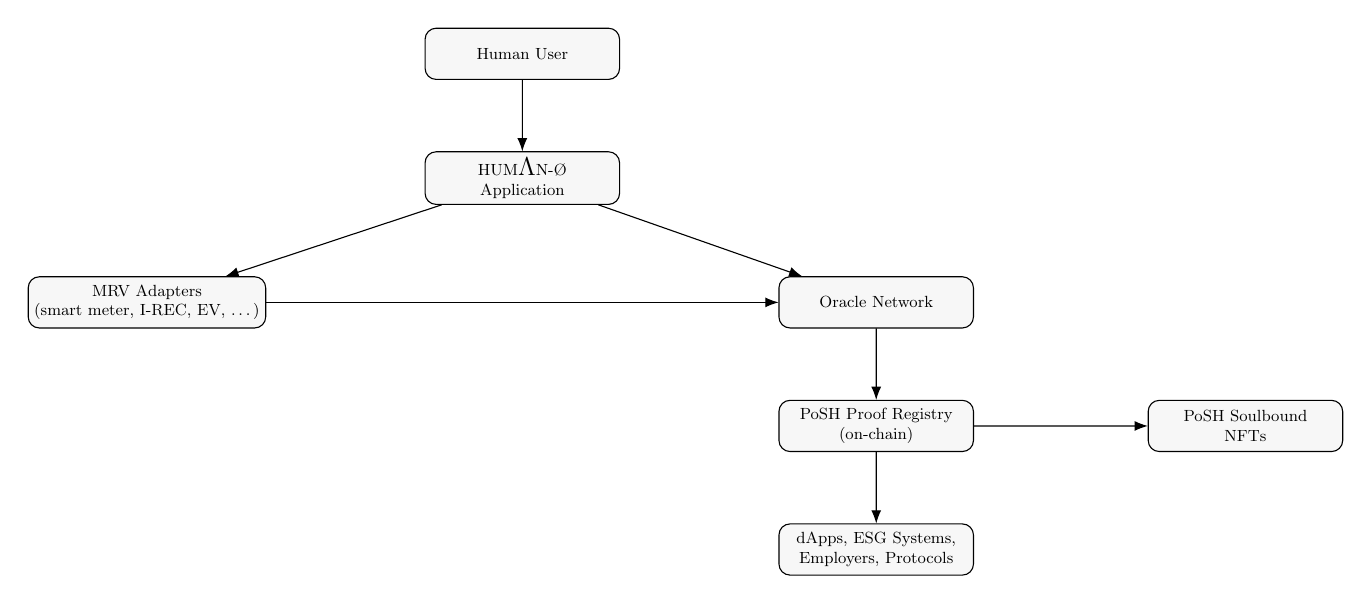
\begin{tikzpicture}[
    scale=0.65,
    transform shape,
    node distance=1.4cm and 2.8cm,
    every node/.style={font=\small},
    box/.style={rectangle, rounded corners, draw, align=center, fill=gray!6, minimum width=3.8cm, minimum height=1cm},
    arrow/.style={-Latex}
  ]

  \node[box] (human) {Human User};
  \node[box, below=of human] (app) {HUM{\Large$\Lambda$}N-Ø\\Application};
  \node[box, below left=of app, xshift=-0.3cm] (mrv) {MRV Adapters\\(smart meter, I-REC, EV, \dots)};
  \node[box, below right=of app, xshift=0.3cm] (oracle) {Oracle Network};
  \node[box, below=of oracle] (registry) {PoSH Proof Registry\\(on-chain)};
  \node[box, right=3.4cm of registry] (nft) {PoSH Soulbound\\NFTs};
  \node[box, below=of registry] (consumers) {dApps, ESG Systems,\\Employers, Protocols};

  \draw[arrow] (human) -- (app);
  \draw[arrow] (app) -- (mrv);
  \draw[arrow] (mrv) -- (oracle);
  \draw[arrow] (app) -- (oracle);
  \draw[arrow] (oracle) -- (registry);
  \draw[arrow] (registry) -- (nft);
  \draw[arrow] (registry) -- (consumers);

  \end{tikzpicture}
  \caption{High-level architecture of the PoSH protocol.}
  \label{fig:posh-architecture}
\end{figure}

\section{Identity Layer (Agnostic and Modular)}

PoSH requires each sustainability proof to be associated with one unique human
being, but it intentionally avoids prescribing any specific identity system.
Instead, PoSH implements a modular, provider-agnostic identity architecture in
which multiple decentralized identity mechanisms can coexist, interoperate, and
be upgraded independently. The protocol receives only a pseudonymous commitment,
never personal data or biometric information.

\subsection{Unified Identity Commitment}

Let $\textsf{IdP}$ denote any identity provider---such as Humanity Protocol,
World ID, Sismo, BrightID, Proof of Humanity, Gitcoin Passport, PolygonID,
Passkeys/WebAuthn, or any W3C-compatible verifiable credential system. Each
provider outputs a proof of uniqueness, membership, or personhood.

PoSH abstracts these systems under a unified commitment:

\[
\mathsf{humanId} = H(\textsf{IdP.output} \parallel \textsf{salt}) \, .
\]

This ensures unlinkability across platforms while permitting the user to switch
identity providers without invalidating past PoSH proofs.

\subsection{Supported Identity Modalities}

PoSH supports diverse identity primitives, including:

\begin{itemize}[leftmargin=*]
  \item \textbf{Zero-knowledge personhood:} World ID, Humanity Protocol,
        Semaphore/RLN, Sismo Vault proofs.
  \item \textbf{Graph-based Sybil resistance:} BrightID, Circles UBI.
  \item \textbf{Verifiable credentials:} PolygonID, Iden3/DID, EAS attestations.
  \item \textbf{Device-bound trust:} WebAuthn/Passkeys, secure enclave
        attestations, local biometrics hashed inside the device.
  \item \textbf{Hybrid multi-signal systems:} Gitcoin Passport, ENS-based
        identity bundles.
\end{itemize}

PoSH remains neutral toward all identity providers and does not require any
specific technology to dominate the identity layer.

\subsection{Identity Requirements}

Each identity solution used with PoSH must satisfy:

\begin{enumerate}[leftmargin=*]
  \item \textbf{Uniqueness:} One human corresponds to one identity commitment.
  \item \textbf{Sybil resistance:} Resistance must come from ZK uniqueness,
        graph proofs, device attestations, biometrics, or multi-signal
        aggregation.
  \item \textbf{Privacy:} Raw identity attributes, biometrics, and credentials
        never leave the provider; only commitments or ZK proofs are used.
  \item \textbf{Non-transferability:} Identity commitments cannot be reassigned
        between different human users.
\end{enumerate}

\subsection{Normalization Layer}

Because providers use heterogeneous proof formats, PoSH defines:

\[
\mathsf{uniqueProof} = \textsf{Normalize}(\textsf{IdP.output})
\]

which standardizes identity proofs into a format suitable for PoSH. This allows
``hot-swapping'' identity providers without affecting PoSH proofs already stored
on-chain.

\subsection{Identity in the UC Model}

In the Universal Composability framework, the identity layer is captured as an
ideal functionality $\mathcal{F}_{\textsf{IdP}}$ that guarantees:

\begin{itemize}[leftmargin=*]
  \item correctness of uniqueness proofs,
  \item unlinkability across identity systems,
  \item modularity and replaceability of providers,
  \item protection against mass deanonymization attacks.
\end{itemize}

PoSH integrates with any $\mathcal{F}_{\textsf{IdP}}$ satisfying these
properties, making the protocol flexible, future-proof, and independent of any
single identity ecosystem.

\section{Impact Verification Layer (MRV $\rightarrow$ Oracle)}

\subsection{Measurement, Reporting, Verification (MRV)}

Each sustainability action is captured by MRV adapters connected to real-world
data sources, including:

\begin{itemize}[leftmargin=*]
    \item smart meters and renewable energy certificates (I-RECs) \cite{khurana2023recBlockchain},
    \item electric vehicle (EV) charging systems,
    \item solar generation and community microgrids \cite{fu2023recCommunity},
    \item low-carbon mobility data,
    \item recycling and waste management attestation systems.
\end{itemize}

The MRV process produces a digitally signed report, denoted
\(\mathsf{mrvReport}\), containing:

\[
\langle \mathsf{type},\, \mathsf{quantity},\, \mathsf{unit},\, \mathsf{co2e},\,
\mathsf{timestamp},\, \mathsf{evidenceRefs} \rangle \; .
\]

\subsection{Oracle Verification Process}

The Oracle Verification process in the Proof of Sustainable Humanity (PoSH) protocol is the crucial step where decentralized Oracle nodes validate the correctness of an incoming Measurable, Reportable, and Verifiable (MRV) report before an on-chain proof is registered. This process ensures that the reported sustainability action is authentic, unique, and plausible.

\subsubsection{How MRV Correctness is Determined}

Oracle nodes perform four specific checks to determine the correctness and integrity of the MRV report:

\begin{enumerate}[label=\arabic*.,leftmargin=*]
    \item \textbf{Data Authenticity and Digital Signatures:}
    The oracle checks the MRV report's digital signature to confirm that the data originated from the expected, trusted source (e.g., a verified IoT device, certified data provider, or a secure application) and has not been tampered with. This confirms who reported the action.

    \item \textbf{Absence of Double Counting:}
    The oracle verifies that the identical sustainability action has not already been reported and committed to the Proof Registry. This is a crucial Sybil resistance and integrity check, often accomplished by checking the uniqueness of the $\mathsf{mrvHash}$ or related commitment data.

    \item \textbf{Consistency with External Trusted Data Sources:}
    The oracle cross-references the reported action with external, trusted data sources. This adds an independent layer of verification. For example, if a renewable energy action is reported, the oracle may check its $\mathsf{impactValue}$ against public energy grid data or meteorological reports for that region and time.

    \item \textbf{Plausibility of Values:}
    The oracle assesses the logical and technical plausibility of the reported $\mathsf{impactValue}$ by comparing it to established device or regional norms. For example, a single residential solar panel claiming to generate an implausibly high amount of energy in a short period would fail this check.
\end{enumerate}

\subsubsection{On-Chain Claim Generation}

Once all four checks are passed, the decentralized oracle network generates a canonical, signed on-chain claim that is submitted to the PoSH smart contract. This claim is created by hashing the key verified data points, which binds the proof to the human identity and the verified action:

\[
\mathsf{claim} = H(\mathsf{humanId} \parallel \mathsf{impactType} \parallel \mathsf{impactValue} \parallel \mathsf{methodologyHash} \parallel \mathsf{mrvHash})
\]

The final claim also includes the oracle's digital signature ($\sigma$) to prove its validation:

\[
\langle \mathsf{humanId}, \mathsf{mrvHash}, \mathsf{methodology}, \mathsf{score} \rangle, \quad \sigma = \mathsf{Sign}_{sk_o}(\mathsf{claim})
\]

\section{On-Chain Proof Registration}

\subsection{Proof Registry}

The \emph{PoSH Proof Registry} contract stores canonical, deduplicated proof
records. Each record contains:

\[
\mathsf{ProofRecord} =
\langle 
\mathsf{humanId},\,
\mathsf{impactType},\,
\mathsf{impactValue},\,
\mathsf{methodologyHash},\,
\mathsf{verificationHash},\,
\mathsf{timestamp}
\rangle \; .
\]

Proofs are immutably linked to a human’s sustainability ledger.

\subsection{PoSH Soulbound Tokens}

Users may optionally mint a \emph{PoSH NFT} representing one or more proof
records. These tokens are soulbound, i.e. non-transferable, and their metadata
contains:

\begin{itemize}[leftmargin=*]
    \item impact categories,
    \item aggregated carbon-equivalent impact,
    \item MRV confidence scores,
    \item methodology identifiers.
\end{itemize}

Minting costs are limited strictly to blockchain network fees.

\section{Zero-Knowledge Privacy Layer}

The PoSH protocol supports optional zero-knowledge proofs (ZKPs) to ensure
privacy while maintaining verifiability.

Two ZK circuits are defined:

\begin{enumerate}[label=\arabic*.,leftmargin=*]
    \item \textbf{Identity circuit:}
    proves that the prover is a member of the human registry without revealing
    the corresponding leaf in the Merkle tree \cite{benSasson2014zkSNARK}.

    \item \textbf{Impact circuit:}
    takes raw MRV data as private input and proves correctness of
    \(\mathsf{impactValue}\) and \(\mathsf{co2e}\) without exposing raw activity.
\end{enumerate}

Thus, a user can prove:
\[
\text{``I performed a valid 5 kWh renewable energy action''}
\]
without revealing meter IDs, timestamps, or location.

\section{Reputation and Scoring}

PoSH introduces an optional reputation mechanism to aggregate sustainability
actions into a numerical score. The reputation contract implements:

\[
\mathsf{score}(h) = \sum_{i \in \mathcal{P}(h)} w_i \cdot \mathsf{impactValue}_i
\]

where \(w_i\) are methodology-dependent weights that may incorporate:

\begin{itemize}[leftmargin=*]
    \item input source reliability,
    \item carbon-equivalent reduction,
    \item MRV confidence and provenance,
    \item temporal decay functions.
\end{itemize}

\section{PoSH as a Cryptographic Primitive}

\subsection{Formal Definition}

Let \(\mathcal{H}\) be a collision-resistant hash function, \(\mathcal{S}\) a
secure digital signature scheme \((\textsf{KeyGen},\textsf{Sign},\textsf{Verify})\),
and \(\Pi_{\textsf{ZK}}\) a zero-knowledge proof system. Let \(\mathbb{U}\) be
the set of unique humans, \(\mathbb{A}\) the set of measurable sustainability
actions, and \(\mathbb{O}\) the set of oracle nodes.

Each human \(u \in \mathbb{U}\) has a persistent pseudonymous identifier:
\[
  \mathsf{humanId}_u = \mathcal{H}(pk_u \parallel \mathsf{uniqueProof}_u)
\]
where \(pk_u\) is a public key and \(\mathsf{uniqueProof}_u\) is a proof of
uniqueness (e.g., from a ZK-identity system).

A sustainability event is represented as:
\[
  E = \langle \mathsf{type},\; v,\; \mathsf{co2e},\; t,\; \mathsf{evidence} \rangle
\]
with quantity \(v\), carbon-equivalent \(\mathsf{co2e}\), timestamp \(t\), and
MRV evidence bundle \(\mathsf{evidence}\). The MRV commitment is:
\[
  \mathsf{mrvHash} = \mathcal{H}(E) \; .
\]

A decentralized oracle network evaluates \(\mathsf{evidence}\) and produces a
signed claim:
\[
  \mathsf{claim} = \langle \mathsf{humanId}_u,\; \mathsf{mrvHash},\;
  \mathsf{methodology},\; \mathsf{score} \rangle , \quad
  \sigma = \textsf{Sign}_{sk_o}(\mathsf{claim})
\]
for some oracle \(o \in \mathbb{O}\).

A \emph{Real-World Action Proof} (RWAP) commitment is defined as:
\[
  \mathsf{RWAP} =
  \mathcal{H}\big(
    \mathsf{humanId}_u \parallel
    \mathsf{mrvHash} \parallel
    \mathsf{methodology} \parallel
    \sigma
  \big) \; .
\]

A PoSH proof is generated by a procedure
\(\textsf{ProvePoSH}(u,E) \rightarrow \mathsf{RWAP}\) and stored in an on-chain
registry. Verification checks (i) the uniqueness proof, (ii) oracle signature
validity, and (iii) non-duplication of \(\mathsf{RWAP}\) in the registry.

\subsection{Security Properties}

We outline the core security properties of PoSH:

\paragraph{Completeness.}
If MRV data is correct, the oracle signatures are valid, and the identity proof
is correct, then a valid PoSH proof produced by an honest prover is always
accepted:
\[
  \Pr[\textsf{VerifyPoSH}(\mathsf{RWAP}) = 1] = 1 \; .
\]

\paragraph{Soundness.}
No probabilistic polynomial-time adversary can forge a PoSH proof for an action
that is not backed by valid MRV and oracle signatures:
\[
  \Pr[\mathcal{A} \text{ forges } \mathsf{RWAP}] \leq \text{negl}(\lambda) \; .
\]

\paragraph{Privacy.}
Zero-knowledge impact proofs ensure that a verifier learns only the exposed
aggregates (e.g., \(\mathsf{co2e}\), methodology) and not the raw MRV data,
under the standard zero-knowledge definition for \(\Pi_{\textsf{ZK}}\).

\paragraph{Non-transferability.}
Because \(\mathsf{humanId}_u\) is bound inside \(\mathsf{RWAP}\), PoSH proofs
are inherently soulbound; transferring them would require forging a new identity
with the same identifier, which is computationally infeasible.

\paragraph{Sybil resistance.}
Sybil attacks are mitigated via unique human proofs, rate limiting per identity,
oracle multisignature requirements, and hash-based MRV deduplication.

\subsection{Comparison with PoW, PoS, and PoA}

\begin{table}[h!]
  \centering
  \begin{tabular}{p{2cm}p{3cm}p{3cm}p{3cm}}
    \hline
    Primitive & Security basis & Externality & Real-world link \\
    \hline
    PoW & Computational hardness & High energy cost & None \\
    PoS & Capital commitment & Low direct cost & None \\
    PoA & Trusted identities & Moderate & Indirect (off-chain) \\
    \textbf{PoSH} & RWAP commitments & \textbf{Positive externality} & \textbf{Direct sustainability actions} \\
    \hline
  \end{tabular}
  \caption{Comparative view of PoSH versus classical consensus primitives.}
\end{table}

PoSH is the first primitive where the ``security budget'' is grounded in
positive real-world externalities (sustainable actions) rather than energy
burn or capital lock-up.

\subsection{Symbolic Protocol Flow and UC-style Model}

Figure~\ref{fig:posh-crypto-flow} illustrates the cryptographic flow of a PoSH
proof, from human action to on-chain commitment.

\begin{figure}[h!]
  \centering
  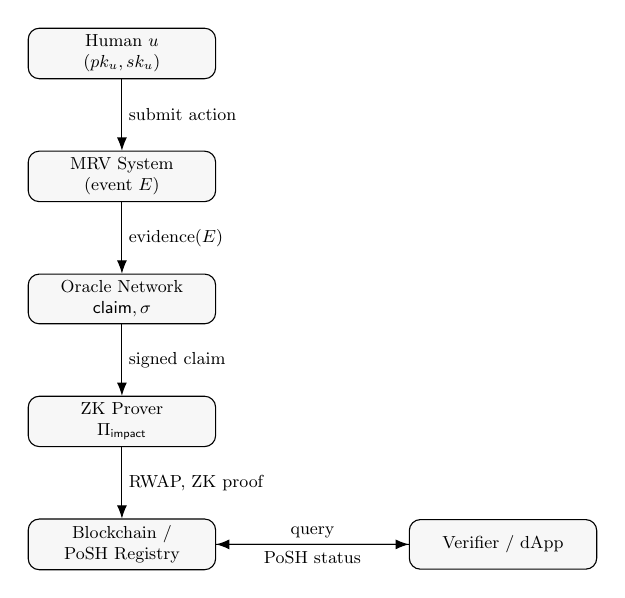
\begin{tikzpicture}[
    scale=0.7,
    transform shape,
    node distance=1.3cm and 2.7cm,
    every node/.style={font=\small},
    box/.style={rectangle, rounded corners, draw, align=center, fill=gray!6,
                minimum width=3.4cm, minimum height=0.9cm},
    arrow/.style={-Latex}
  ]

  \node[box] (u) {Human $u$\\($pk_u, sk_u$)};
  \node[box, below=of u] (mrv) {MRV System\\(event $E$)};
  \node[box, below=of mrv] (oracle) {Oracle Network\\$\mathsf{claim}, \sigma$};
  \node[box, below=of oracle] (zk) {ZK Prover\\$\Pi_{\textsf{impact}}$};
  \node[box, below=of zk] (chain) {Blockchain /\\PoSH Registry};
  \node[box, right=3.5cm of chain] (verifier) {Verifier / dApp};

  \draw[arrow] (u) -- node[right]{submit action} (mrv);
  \draw[arrow] (mrv) -- node[right]{evidence$(E)$} (oracle);
  \draw[arrow] (oracle) -- node[right]{signed claim} (zk);
  \draw[arrow] (zk) -- node[right]{RWAP, ZK proof} (chain);
  \draw[arrow] (verifier) -- node[above]{query} (chain);
  \draw[arrow] (chain) -- node[below]{PoSH status} (verifier);

  \end{tikzpicture}
  \caption{Cryptographic flow of a PoSH proof from MRV to on-chain RWAP.}
  \label{fig:posh-crypto-flow}
\end{figure}

For a UC-style abstraction, we consider an ideal functionality
\(\mathcal{F}_{\textsf{PoSH}}\) that maintains a registry of valid sustainability
commitments and enforces uniqueness and soundness properties. The environment
\(\mathcal{Z}\) interacts with honest parties and an adversary \(\mathcal{A}\),
and the real-world PoSH protocol \(\Pi_{\textsf{PoSH}}\) is required to emulate
\(\mathcal{F}_{\textsf{PoSH}}\) in the standard UC sense.

\begin{figure}[h!]
  \centering
  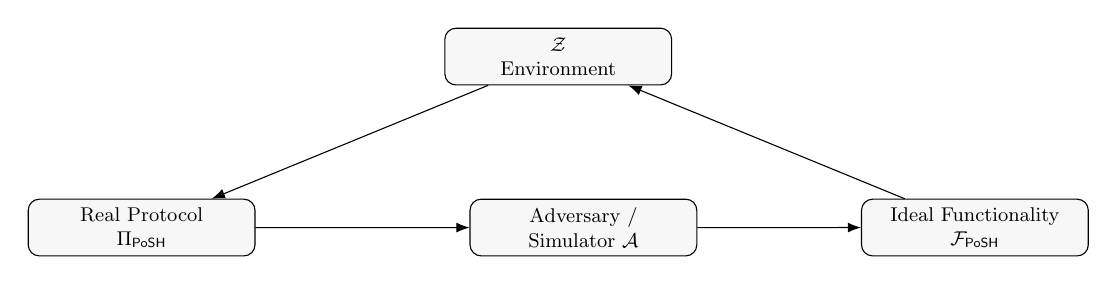
\begin{tikzpicture}[
    scale=0.8,
    transform shape,
    node distance=1.8cm and 3.0cm,
    every node/.style={font=\small},
    box/.style={rectangle, rounded corners, draw, align=center, fill=gray!6,
                minimum width=3.6cm, minimum height=0.9cm},
    arrow/.style={-Latex}
  ]

  \node[box] (env) {$\mathcal{Z}$\\Environment};
  \node[box, below left=of env] (proto) {Real Protocol\\$\Pi_{\textsf{PoSH}}$};
  \node[box, below right=of env] (ideal) {Ideal Functionality\\$\mathcal{F}_{\textsf{PoSH}}$};
  \node[box, right=3.4cm of proto] (adv) {Adversary /\\Simulator $\mathcal{A}$};

  \draw[arrow] (env) -- (proto);
  \draw[arrow] (proto) -- (adv);
  \draw[arrow] (adv) -- (ideal);
  \draw[arrow] (ideal) -- (env);

  \end{tikzpicture}
  \caption{UC-style view of the PoSH protocol and ideal functionality
           $\mathcal{F}_{\textsf{PoSH}}$.}
  \label{fig:posh-uc-model}
\end{figure}

\section{Conclusion}

PoSH is proposed as a foundational cryptographic primitive for representing
human-scale sustainability contributions. By integrating MRV, decentralized
oracles, privacy-preserving cryptography, and transparent on-chain registries,
PoSH enables a future where positive environmental actions can be verified,
recognized, and composed into digital identity systems without compromising
individual privacy or equity.

This chapter establishes PoSH as a viable alternative consensus dimension for
sustainability-centric digital systems, offering a means for humanity to align
its digital infrastructure with planetary boundaries.

\chapter{Related Work}
\label{chap:related}

Although no prior work proposes a system equivalent to Proof of Sustainable
Humanity (PoSH), several research lines and existing protocols motivate and
contextualize its design. These can be grouped into three domains:
proof-of-personhood, self-sovereign identity (SSI), and blockchain-based
sustainability verification.

\section{Proof of Personhood and Human Uniqueness}

Multiple projects aim to establish provable human uniqueness as a Sybil
resistance mechanism. Examples include World ID (Worldcoin), which relies on
privacy-preserving biometric nullifiers \cite{worldcoinWhitepaper}, and Idena,
an early PoP protocol analyzed in depth in \cite{ohlhaver2025compressed}. Other
initiatives explore KYC-free proof-of-personhood through decentralized graphs
or attestations, such as Polkadot's Project Individuality
\cite{polkadot2025individuality} or BrightID. These systems attempt to provide
digital human uniqueness without central authority, forming a relevant precursor
to PoSH’s identity abstraction model.

\section{Self-Sovereign Identity (SSI)}

The principles of self-sovereign identity (SSI)—control, consent, portability,
and privacy—are discussed extensively in the literature, including systematic
reviews by Schardong and Custódio \cite{schardong2022ssiSurvey} and Pava-Díaz
et al. \cite{pava2024ssiBlockchain}. Threat modeling for SSI protocols is
analyzed in \cite{pohn2024ssiThreats}. PoSH builds on these foundations while
remaining intentionally agnostic to any single identity provider: any system
capable of generating a uniqueness proof compatible with
$\mathsf{humanId} = H(\textsf{IdP.output} \parallel \textsf{salt})$ can be used.

\section{Blockchain-Based Sustainability and MRV}

Tokenizing sustainability attributes—such as renewable energy certificates
(RECs), carbon credits, or MRV-based environmental claims—has been explored in
multiple blockchain proposals, including privacy-preserving REC trading
\cite{energy2024recTrading}, decentralized community energy markets
\cite{fu2023recCommunity}, and registry modernization efforts
\cite{infosys2025blockchainREC,heliyon2025indonesiaREC}. However, these systems
lack any intrinsic link to human identity or personal sustainability actions.
PoSH introduces a new concept: real-world action proofs (RWAP) bound to unique
human identities, enabling sustainability to become a cryptographic primitive
in human-centered digital systems.


% =====================================================
% Appendix A — Threat Model and Adversaries
% =====================================================

\appendix
\chapter{Threat Model and Adversaries}
\label{appendix:threat-model}

This appendix formalizes the threat environment in which the PoSH protocol
operates. We distinguish between classes of adversaries, their capabilities,
and the security properties the protocol is designed to guarantee.

\section{Adversarial Goals}

An adversary $\mathcal{A}$ interacting with PoSH may attempt to:

\begin{enumerate}[label=\arabic*.,leftmargin=*]
  \item \textbf{Forge sustainability events:} fabricate an MRV record or alter
        measurement values to claim non-existent impact.
  \item \textbf{Exploit the oracle layer:} compromise oracle keys, inject
        fraudulent claims, or censor valid submissions.
  \item \textbf{Perform identity-based attacks:} create multiple identities
        (Sybil attack), impersonate legitimate users, or transfer PoSH proofs
        between identities.
  \item \textbf{Break privacy guarantees:} infer sensitive behavioral or
        geolocation data from public PoSH proofs.
  \item \textbf{Manipulate reputation systems:} artificially inflate sustainability
        scores through repeated, low-value events or oracle collusion.
  \item \textbf{Disrupt chain-level finality:} reorder, remove, or censor proof
        registrations on-chain.
\end{enumerate}

\section{Adversary Model}

We consider the following adversary classes:

\subsection{Class A: Local Malicious User}
Capabilities include:

\begin{itemize}[leftmargin=*]
  \item forging local sensor data,
  \item replaying MRV events,
  \item colluding with untrusted MRV sources,
  \item probing the identity layer for collision vulnerabilities.
\end{itemize}

Mitigations:
\begin{itemize}[leftmargin=*]
  \item cryptographic signatures on MRV,
  \item deduplication via $\mathsf{mrvHash}$,
  \item ZK-unique identity proofs,
  \item time-locked and device-bound attestations.
\end{itemize}

\subsection{Class B: Compromised Oracle}
Capabilities:

\begin{itemize}[leftmargin=*]
  \item emit fraudulent $\mathsf{claim}$ values,
  \item collude with users to create false-positive impact,
  \item censor legitimate MRV events.
\end{itemize}

Mitigations:
\begin{itemize}[leftmargin=*]
  \item multisignature oracle committees,
  \item stake-slashable oracle sets,
  \item duplicated data ingest from heterogenous MRV providers.
\end{itemize}

\subsection{Class C: Global Passive Adversary}
Capabilities:

\begin{itemize}[leftmargin=*]
  \item network-wide traffic surveillance,
  \item timing correlation between MRV events and identities,
  \item linking of PoSH proofs to external metadata.
\end{itemize}

Mitigations:
\begin{itemize}[leftmargin=*]
  \item ZK privacy layer for MRV,
  \item timing obfuscation and proof batching,
  \item humanId salted commitments.
\end{itemize}

\subsection{Class D: Chain-level Adversary}
Capabilities:

\begin{itemize}[leftmargin=*]
  \item reordering or censoring registry writes,
  \item controlling block producers for MEV-like manipulation,
  \item chain forks or state rewrites.
\end{itemize}

Mitigations:
\begin{itemize}[leftmargin=*]
  \item proof finality dependent on underlying L1 consensus,
  \item verifiable delay before reputation updates,
  \item hash-anchoring PoSH commitments across multiple chains.
\end{itemize}

\subsection{Class E: Systemic Collusion Attack}
Capabilities:

\begin{itemize}[leftmargin=*]
  \item coordinated manipulation between MRV, oracles, and users,
  \item bulk fabrication of greenwashing records,
  \item capture of governance around methodologies.
\end{itemize}

Mitigations:
\begin{itemize}[leftmargin=*]
  \item diversified oracle sets with rotating keys,
  \item open-source, auditable methodologies,
  \item meta-proofs that bind $\mathsf{methodologyHash}$ to published standards.
\end{itemize}

\section{Security Guarantees}

PoSH guarantees, under the assumed hardness of $\mathcal{H}$, $\mathcal{S}$,
and $\Pi_{\textsf{ZK}}$:

\begin{itemize}[leftmargin=*]
  \item \textbf{Soundness:} Only valid, verified sustainability actions can be
        committed on-chain.
  \item \textbf{Uniqueness:} One human $\rightarrow$ one PoSH identity.
  \item \textbf{Non-transferability:} PoSH proofs cannot be reassigned.
  \item \textbf{Privacy:} Raw MRV data cannot be inferred from commitments.
  \item \textbf{Robustness:} The system is resilient against colluding oracles.
  \item \textbf{Liveness:} Honest actions eventually register, despite adversarial
        network conditions.
\end{itemize}

\section{Residual Risks}

Residual attack surfaces include:

\begin{itemize}[leftmargin=*]
  \item MRV corruption by physical tampering,
  \item black-box ML manipulation on sensors,
  \item oracle cartelization,
  \item chain-level governance capture,
  \item large-scale behavioral deanonymization via public metadata.
\end{itemize}

PoSH minimizes but does not eliminate these risks; further mitigation is
possible through cross-chain anchoring, multi-layer proof aggregation, and
hardware-secured MRV attestations.

\chapter*{End of Appendix A}
\addcontentsline{toc}{chapter}{Appendix: Threat Model and Adversaries}
% =====================================================
% Appendix B — Universal Composability (UC) Specification of PoSH
% =====================================================

\chapter{Universal Composability Specification of PoSH}
\label{appendix:uc-model}

This appendix provides a formal definition of the PoSH protocol in the Universal
Composability (UC) framework. We specify the ideal functionality
$\mathcal{F}_{\textsf{PoSH}}$, the real-world protocol $\Pi_{\textsf{PoSH}}$,
the simulator $\mathcal{S}$, and the environment $\mathcal{Z}$ that interacts
with the system.

Our goal is to show that the real-world execution of PoSH securely emulates the
ideal functionality in the UC sense.

\section{The Universal Composability Framework}

The framework of Universal Composability (UC) \cite{Canetti01} is a general-purpose model for the
analysis of cryptographic protocols. It guarantees very strong security
properties. Protocols remain secure even if arbitrarily composed with other
instances of the same or other protocols. Security is defined in the sense of
protocol emulation. Intuitively, a protocol is said to emulate another one if no
environment (observer) can distinguish the executions. Literally, the protocol
may simulate the other protocol (without having access to the code). The notion
of security is derived by implication. Assume a protocol $P_1$ is secure per
definition. If another protocol $P_2$ emulates protocol $P_1$ such that no
environment tells apart the emulation from the execution of the protocol, then
the emulated protocol $P_2$ is as secure as protocol $P_1$.

\subsection{Ideal Functionality}

An ideal functionality is a protocol in which a trusted party that can
communicate over perfectly secure channels with all protocol participants
computes the desired protocol outcome. We say that a cryptographic protocol that
cannot make use of such a trusted party fulfills an ideal functionality if the
protocol can emulate the behavior of the trusted party for honest users, and if
the view that an adversary learns by attacking the protocol is indistinguishable
from what can be computed by a simulator that only interacts with the ideal
functionality.

\subsection{Computation Model}

The computation model of universal composability is that of interactive Turing
machines that can activate each other by writing on each other's communication
tapes. An interactive Turing machine is a form of multi-tape Turing machine and
is commonly used for modelling the computational aspects of communication
networks in cryptography.

\subsection{Communication Model}

The communication model in the bare UC framework is very basic. The messages of
a sending party are handed to the adversary who can replace these messages with
messages of his own choice that are delivered to the receiving party. This is
also the Dolev–Yao threat model (based on the computational model all parties
are modeled as interactive Turing machines).

All communication models that add additional properties such as confidentiality,
authenticity, synchronization, or anonymity are modeled using their own ideal
functionality. An ideal communication functionality takes a message as input and
produces a message as output. The (more limited) powers for the adversary
$\mathcal{A}$ are modeled through the (limited) capacity of the adversary to
interact with this ideal functionality.

\subsubsection{Ideal Authenticated Channel}

For an optimal ideal authenticated channel, the ideal functionality
$\mathcal{F}_{\mathsf{Auth}}$ takes a message $m$ from a party with identity $P$
as input, and outputs the same message together with the identity $P$ to the
recipient and the adversary. To model the power of the adversary to delay
asynchronous communication the functionality $\mathcal{F}_{\mathsf{Auth}}$ may
first send a message to the adversary $\mathcal{A}$ and would only deliver the
message $m,P$ once it receives the command to do so as a reply.

\subsubsection{Ideal Secure Channel}

In an ideal secure channel, the ideal functionality $\mathcal{F}_{\mathsf{Sec}}$
only outputs the identity of the sender to both the recipient and the adversary,
while the message is only revealed to the recipient. This models the requirement
that a secure channel is both authenticated and private. To model some leakage
about the information that is being transferred, $\mathcal{F}_{\mathsf{Sec}}$
may reveal information about the message to the adversary, e.g. the length of
the message. Asynchronous communication is modeled through the same delay
mechanism as for $\mathcal{F}_{\mathsf{Auth}}$.

\subsubsection{Ideal Anonymous and Pseudonymous Channels}

While the technical means, and the physical assumptions behind anonymous and
pseudonymous communication are very different, the modeling of such channels
using ideal functionalities is analogous.

In an ideal anonymous channel, the ideal functionality $\mathcal{F}_{\mathsf{Anon}}$
takes a message $m$ from a party with identity $P$ as input, and outputs the
same message but without disclosing the identity $P$ to the recipient and the
adversary.

In an ideal pseudonymous channel, the participating parties first register
unique pseudonyms with the ideal functionality $\mathcal{F}_{\mathsf{Pseu}}$. To
do a transfer $\mathcal{F}_{\mathsf{Pseu}}$ takes a message $m$ and the
pseudonym $nym$ of the recipient as input. The ideal functionality looks up the
owner of the pseudonym and transfers the message $m,nym$ without revealing the
identity of the sender.

\subsection{Impossibility Results and Setup Assumptions}

There exists no bit commitment protocol that is universally composable in the
standard model of cryptography. The intuition is that in the ideal model, the
simulator has to extract the value to commit to from the input of the
environment. This would allow the receiver in the real protocol to extract the
committed value and break the security of the protocol. This impossibility
result can be applied to other functionalities.

To circumvent the above impossibility result, additional assumptions are
required. Additional setup and trust assumptions, such as the common reference
string model and the assumption of a trusted certification authority are also
modeled using ideal functionalities in UC.

\section{Ideal Functionality \texorpdfstring{$\mathcal{F}_{\textsf{PoSH}}$}{F-PoSH}}

The ideal functionality maintains a registry of valid sustainability proofs and
enforces uniqueness, soundness, and privacy guarantees.

\subsection*{State Variables}

$\mathcal{F}_{\textsf{PoSH}}$ maintains:

\begin{itemize}[leftmargin=*]
  \item $\mathsf{Users}$: a map of human identifiers to public keys,
  \item $\mathsf{MRV}$: a list of submitted MRV commitments,
  \item $\mathsf{Claims}$: a list of oracle-verified claims,
  \item $\mathsf{Registry}$: the set of valid PoSH commitments,
  \item $\mathsf{Revoked}$: a set of invalidated, fraudulent, or outdated proofs.
\end{itemize}

\subsection*{Initialization}

On initialization, $\mathcal{F}_{\textsf{PoSH}}$ sets all sets/maps to empty
and notifies the adversary $\mathcal{A}$.

\subsection*{Interfaces}

\paragraph{Register User.}

Upon receiving $(\textsf{register}, pk, \mathsf{uniqueProof})$ from a party $U$:

\begin{enumerate}[leftmargin=*]
  \item Verify the uniqueness proof.
  \item If valid, compute $\mathsf{humanId} = H(pk \parallel \mathsf{uniqueProof})$.
  \item Store $(\mathsf{humanId}, pk)$ in $\mathsf{Users}$.
  \item Return $(\textsf{registered}, \mathsf{humanId})$ to $U$.
\end{enumerate}

\paragraph{Submit MRV Event.}

Upon receiving $(\textsf{mrv\_submit}, \mathsf{humanId}, E)$:

\begin{enumerate}[leftmargin=*]
  \item Compute $\mathsf{mrvHash} = H(E)$.
  \item If $\mathsf{mrvHash}$ already exists, reject.
  \item Store $(\mathsf{humanId}, \mathsf{mrvHash}, E)$ in $\mathsf{MRV}$.
  \item Notify oracles in the ideal world.
\end{enumerate}

\paragraph{Oracle Claim.}

Given a valid MRV event, an ideal oracle sends:

$(\textsf{oracle\_claim}, \mathsf{humanId}, \mathsf{mrvHash}, \mathsf{methodology}, \mathsf{score})$.

$\mathcal{F}_{\textsf{PoSH}}$ checks:

\begin{enumerate}[leftmargin=*]
  \item The MRV event exists.
  \item The methodology and score are well-formed.
\end{enumerate}

Then it stores the claim.

\paragraph{Finalize PoSH Proof.}

Upon receiving $(\textsf{prove\_posh}, \mathsf{humanId}, \mathsf{mrvHash})$:

\begin{enumerate}[leftmargin=*]
  \item Check the claim exists in $\mathsf{Claims}$.
  \item Compute $\mathsf{RWAP} = H(\mathsf{humanId}, \mathsf{mrvHash}, \mathsf{methodology})$.
  \item Store in $\mathsf{Registry}$.
  \item Return $(\textsf{posh\_proof}, \mathsf{RWAP})$ to $U$.
\end{enumerate}

\paragraph{Verify Proof.}

On query $(\textsf{verify}, \mathsf{RWAP})$:

\[
  \textsf{Return } 
  \begin{cases}
  \textsf{valid}, & \mathsf{RWAP} \in \mathsf{Registry} \land \mathsf{RWAP} \notin \mathsf{Revoked} \\
  \textsf{invalid}, & \text{otherwise.}
  \end{cases}
\]

\section{Real-World Protocol \texorpdfstring{$\Pi_{\textsf{PoSH}}$}{Pi-PoSH}}

The real-world protocol consists of several interacting components:

\begin{itemize}[leftmargin=*]
  \item Users generating MRV evidence and running ZK circuits,
  \item MRV devices producing signed raw evidence,
  \item Oracle networks verifying MRV correctness and emitting signatures,
  \item Smart contracts maintaining the on-chain PoSH registry.
\end{itemize}

\subsection*{Protocol Steps}

\paragraph{1. Identity Generation.}

User generates $(pk, sk)$ and produces a ZK-unique proof:

\[
  \Pi_{\textsf{unique}}(pk) \rightarrow \mathsf{uniqueProof}
\]

Then calls the smart contract to register.

\paragraph{2. MRV Submission.}

User collects MRV evidence from real-world devices and submits:

\[
  \mathsf{mrvHash} = H(E)
\]

to the oracle network.

\paragraph{3. Oracle Attestation.}

Oracles validate $E$, produce a signed claim:

\[
  \sigma = \mathsf{Sign}_{sk_o}(\mathsf{claim})
\]

and write to the chain.

\paragraph{4. ZK Impact Proof.}

User produces:

\[
  \Pi_{\textsf{impact}}(E)
\]

and requests registry entry.

\paragraph{5. Registry Entry.}

Smart contract computes:

\[
  \mathsf{RWAP} = H(\mathsf{humanId}, \mathsf{mrvHash}, \mathsf{methodology}, \sigma)
\]

and stores it.

\section{Simulator \texorpdfstring{$\mathcal{S}$}{S}}

To prove UC security, we construct a simulator $\mathcal{S}$ that interacts with
the ideal functionality and the environment such that the environment cannot
distinguish between ideal and real executions.

\subsection*{Capabilities of the Simulator}

The simulator:

\begin{itemize}[leftmargin=*]
  \item intercepts oracle messages,
  \item emulates smart contract events,
  \item simulates MRV and ZK proofs,
  \item ensures no adversary learns private data,
  \item extracts adversarial MRV commitments to detect forgeries.
\end{itemize}

\subsection*{Simulation Strategy}

\begin{enumerate}[label=\arabic*.,leftmargin=*]
  \item \textbf{User Registration:}  
    $\mathcal{S}$ forwards $(pk, \mathsf{uniqueProof})$ to $\mathcal{F}_{\textsf{PoSH}}$.
  \item \textbf{MRV Submission:}  
    $\mathcal{S}$ receives adversarial $E$ and extracts $\mathsf{mrvHash}$.
  \item \textbf{Oracle Claims:}  
    $\mathcal{S}$ fabricates signatures consistent with ideal claims.
  \item \textbf{RWAP Creation:}  
    Whenever the adversary attempts to create $\mathsf{RWAP}$,  
    $\mathcal{S}$ queries $\mathcal{F}_{\textsf{PoSH}}$ to validate.
  \item \textbf{Verification Queries:}  
    $\mathcal{S}$ relays all $\textsf{verify}$ queries to $\mathcal{F}_{\textsf{PoSH}}$.
\end{enumerate}

Thus, the simulator can replicate all adversarial views without access
to private MRV data or ZK inputs.

\section{Security Theorem}

\begin{theorem}
Under the assumed hardness of $\mathcal{H}$, security of the digital signature
scheme $\mathcal{S}$, and zero-knowledge and soundness of the ZK systems
$\Pi_{\textsf{unique}}$ and $\Pi_{\textsf{impact}}$, the PoSH protocol
$\Pi_{\textsf{PoSH}}$ UC-emulates the ideal functionality
$\mathcal{F}_{\textsf{PoSH}}$.
\end{theorem}

\begin{proof}[Proof Sketch.]
For any real-world adversary $\mathcal{A}$ interacting with
$\Pi_{\textsf{PoSH}}$, we construct a simulator $\mathcal{S}$ such that no
environment $\mathcal{Z}$ can distinguish between the real execution and the
ideal execution.

Key points:
\begin{itemize}[leftmargin=*]
  \item ZK proofs hide MRV event details, so $\mathcal{S}$ can simulate them.
  \item Oracle signatures are simulated by $\mathcal{S}$ using ideal claims.
  \item The ideal registry ensures soundness; real and ideal behaviors agree.
  \item Unique human proofs prevent identity-based adversarial deviations.
\end{itemize}

Thus, $\Pi_{\textsf{PoSH}}$ UC-emulates $\mathcal{F}_{\textsf{PoSH}}$.
\end{proof}

\chapter*{End of Appendix B}
\addcontentsline{toc}{chapter}{Appendix B: UC Specification of PoSH}



\bibliographystyle{alpha}
\bibliography{refs}

\end{document}

